\section{Case Study}

To illustrate some aspects of RCloud, we present an example application
for stock price analysis.\footnote{Unfortunately this report could not
include production notebooks containing proprietary or personal information.}
The example, although simplified, shows key steps in the development
and deployment process we support.

\begin{figure}
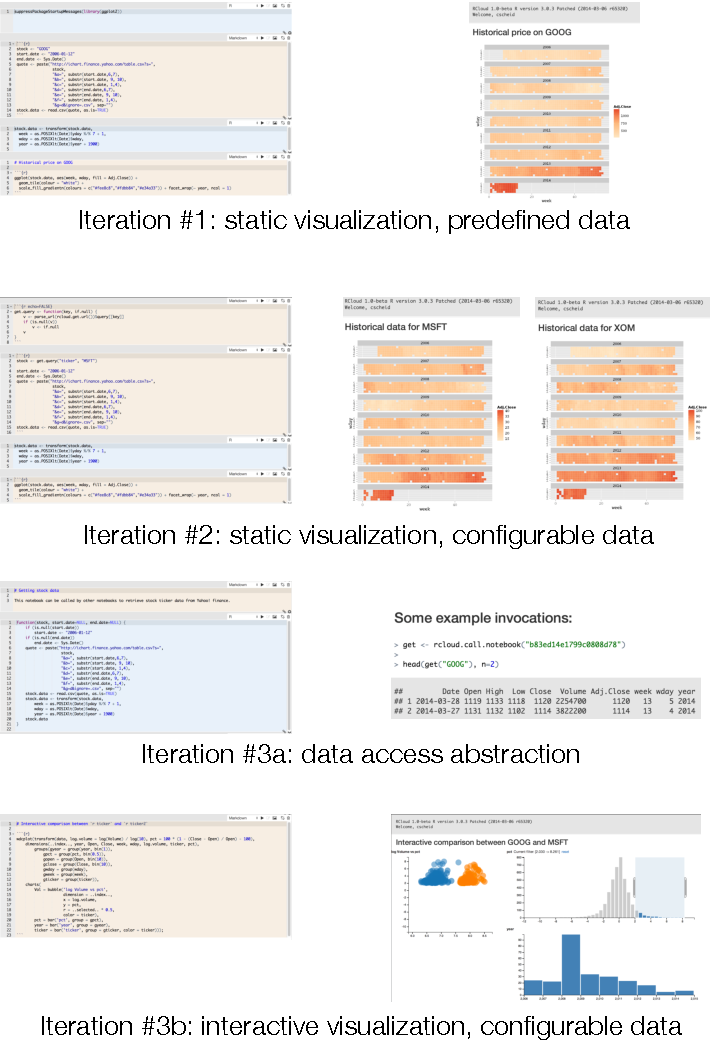
\includegraphics[width=\linewidth]{fig/casestudy1/casestudy1.pdf}
\caption{\label{fig:stockvis}Iterations of a stock ticker
  visualization, based on an example by Hadley Wickham. A
  simple, static visualization of the closing price of a single stock
  is progressively developed into a configurable display suitable
  for dashboarding, then into an interactive visualization for 
  comparing the volatility and volume of two stocks, and finally
  into an API for data access by other RCloud notebooks. The notebooks
  in this example can all be loaded as web pages. When a notebook
  corresponding to a function call is displayed a web page,
  its associated documentation is displayed.}
\end{figure}

It shows a sequence of visualizations of the performance
of financial stocks over a multi-year period. The first visualization
in this example uses ggplot2 and was written by Hadley Wickham.
It reads data provided by Yahoo! Finance as a web service, and shows
the price for a single trading symbol.

The webpage that produces that visualization includes a link back to
the underlying source code. From this link, a user can fork the notebook.
In the example,a configurable ticker is added, based on the URL of
the notebook. The change to the notebook is very minor.

Next, the notebook author or a collaborator may decide to extend
the application to also provide convenient access to the data,
apart from its visualization.
This is done by creating a notebook that defines a function.
That notebook then becomes a \emph{subroutine} for other notebooks.
It can be invoked from interactive notebooks, such as dashboards.
The data access notebook is version-controlled like other notebooks.

Finally, consider the situation where an analyst wants to understand
the price dynamics of stocks with respects to various attributes and
time ranges. For this, interactive visualization may be very helpful.
In our example, the analyst creates an interactive tool with multiple
linked views.

Through the tight integration of R and JavaScript functions and data,
the analyst writes a function in R which passes the dataframe and the
description of the charts to the dcplot library.  Simple R expressions
are captured as trees to generate JavaScript expressions.  The terse
chart description language, with intelligent defaults inspired by
ggplot2, provides a simple yet powerful interface to the grouping
and reduction functionality of the well-accepted charting libraries
crossfilter, dc.js and d3.js.

% \subsection{Text analysis\label{sec:textvis}}
% Same.

% IMPORTANT: what is unique about RCloud here
% From prototyping to dashboard
% Getting other information from the web
%
